\chapter{Програмне середовище моделювання нелінійних динамічних систем ``qontrol''}
\label{chapter_qontrol}

\section{Аналіз існуючих систем}%%{{{1 ------------------------------------- --------

\paragraph{Matlab, simulink}

Цей комерційний продукт є стандартом де-факто в дослідницьких
роботах в задачах моделювання динамічних систем, а також
багатьох інших областях. Серед позитивних особливостей слід
відзначити наявність великої кількості пакетів для вирішення
різноманітних задач, розвинену, хоч і трохи обмежену мову
програмування, підтримка множини обчислювальних платформ. З
недоліків слід зазначити помітне нав'язування досліднику
методів і прийомів роботи, приховування від користувача деталей
застосовуваних алгоритмів, непомірну вартість, обмежені
можливості роботи з обладнанням.


\paragraph{Scilab, octave}

Є Open-source аналогами Matlab, мають практично сумісну
мову програмування, набір базових можливостей і
пакетів. Відрізняються помітно меншою кількістю доступних
пакетів, що досить добре перекривається відкритістю
платформи, що дозволяє з меншими зусиллями реалізовувати свої
розширення. Безкоштовність, відкритість і вільна ліцензія (CeCILL,
GPLv3+) представляють серйозні переваги для дослідника. Проте,
сумісність з Matlab має і зворотну сторону, а саме обмеженість
мови і нав'язування прийомів роботи.

\paragraph{Multisim}

Спеціальний комерційний продукт, призначений для моделювання,
проектування та аналізу переважно електронних схем. Завдяки
великій базі електронних компонентів і застосування
спеціальних алгоритмів помітно спрощує розробку і моделювання
саме електронних пристроїв. Наявність набору ``ідеальних''
елементів, що застосовуються в теорії управління,
дозволяє в якійсь мірі розширити коло задач за межі
електронного моделювання. Проте, цей продукт залишається
вузькоспеціалізованим засобом. Більш того, закритість і
обмеженість засобів настройки застосовуваних алгоритмів
моделювання не дає в окремих випадках ні отримати адекватний
результат, ні визначити точно причину такої поведінки.

\paragraph{LabView}

Ще один комерційний продукт, який вживається переважно для моделювання
та аналізу електронних схем. Відмінною особливістю даного
продукту є розвинені засоби взаємодії з реальними вимірювальним
приладами та виконавчими механізмами. При цьому, список таких
зовнішніх пристроїв визначається обмеженим набором виробників,
і застосування власних розробок в цьому пакеті можливо, якщо
створюється пристрій, який симулює один зі стандартних. Це істотно
знижує можливість застосування даного пакета при взаємодії з
нестандартним обладнанням.



\paragraph{Висновки}

Таким чином, для проведення досліджень, пов'язаних з вирішенням
поставлених проблем, потрібна розробка як спеціального
програмного забезпечення, так і взаємодіючих з ним апаратних
вимірювальних засобів.



% }}}1


\section{Основи побудови програмного середовища} % {{{1 ------------------------------

Для розробки комплексу ``qoubtol''~\cite{atu_asau26,atu_asau27}
в якості базової мови було обрано C++,
який забезпечує поєднання гнучкості і можливостей розробки
з необхідною швидкістю обчислень. Також, дана мова є цілком
прийнятною для програмування мікроконтролерів класу STM32, що
входять до складу апаратної частини комплексу.

Проте, для реалізації можливостей автоматизації всередині самої
програми, потрібне застосування мови, що не потребує попередньої
компіляції, досить поширеної, відносно швидкої, яка підтримує об'єктну
модель. Як якості такої мови був обраний ECMAScript, відомий також як JavaScript.

\subsection{Реалізація інтроспекції і об'єктної моделі} % {{{2

Для реалізації задач гнучкого підходу до моделювання,
автоматизації та автоматичного побудови інтерфейсних елементів
потрібне отримання інформації про об'єкти системи моделювання
в процесі роботи програми (інтроспекції). У самій мові C++ в
даний момент немає вбудованих засобів реалізації інтроспекції. Бібліотека
Qt, яка використовується в розробці, надає базові можливості
інтроспекції, за рахунок використання метакомпілятора ``moc''.

Для того, щоб скористатися інтроспекцією за допомогою засобів
Qt, необхідно реалізовувати власні класи у вигляді відкритих
спадкоємців класу QObject, та додати спеціальне ключове слово ``Q\_OBJECT''
в опис класу. Після цього з'являється можливість замість
звичайних членів даних класу створювати ``властивості'' (property),
використовуючи ключове слово метакомпілятора ``Q\_PROPERTY'',
наприклад:\\
\verb!Q_PROPERTY( double omega READ getOmega WRITE setOmega );!\\
Після цього можна з програми отримати імена і типи заданих таким
чином властивостей, отримати значення за допомогою функції
``property'', встановити значення за допомогою функції ``setProperty'',
отримати доступ як до властивості об'єкта вбудованої мови
JavaScript. Функції-члени стають видимими для програм на JavaScript після
використання ключового слова ``Q\_INVOKABLE''. Увесь необхідний для
цього програмний код генерується метакомпілятором автоматично.

Проте, безпосереднє використання даного виду інтроспекції не є
зручним при вирішенні задачі моделювання складних динамічних систем. В
першу чергу, доступ до властивостей за допомогою функцій
``property'', ``setProperty'' значно повільніше, ніж безпосередній доступ
або ж доступ за допомогою покажчика або посилання. В процесі
моделювання доступ до властивостей потрібен постійно, і з
урахуванням кількості ітерацій, що досягає десятків мільйонів,
швидкість доступу має вирішальне значення.

Існує також ще один важливий недолік підходу до визначення
властивостей в Qt. До властивості не можна приєднувати довільні
дані користувача. У свою чергу, ці дані необхідні для опису
властивостей параметрів динамічних елементів, наприклад,
мінімальне і максимальне значення, особливості відображення
(або ж приховування) значення параметра елементами інтерфейсу,
необхідність збереження цього параметра під час запису в файл
і так далі. З іншого боку, реалізація доступу до функцій-членів
реалізована коректно, додаткові можливості не потрібні.

Тому, для реалізації всіх вимог, для членів даних був
реалізований окремий підхід до інтроспекції. Для цього
використовувалися можливості як мови C ++, так і
препроцесору. В якості базового класу для подання властивостей
створений клас ``HolderData''. Він є відкритим спадкоємцем
класу ``QAbstractItemModel''. Це дозволяє для доступу до елементів
використовувати стандартний для Qt підхід з використанням
технології ``Model--View''. Для класу створено множину спадкоємців
(HolderInt, HolderDouble, HolderString, HolderFont, HolderDoubleArray \ldots), призначених для
зберігання різноманітних типів даних. Для кожного такого
класу реалізований набір функцій і операторів перетворення
таким чином, що б забезпечити прямий доступ до даних з функцій
класу без накладних витрат, як з боку користувача, так і з боку
компілятора. Також реалізовані функції перетворення в найбільш
часто використовувані типи.

Для того, щоб забезпечити оголошення властивостей практично
таким же способом, як і оголошення звичайних членів даних,
створено набір макросів. При цьому, можна задати довільну
кількість додаткових даних.
Приклад:\\
\verb!PRM_DOUBLE( omega,  efRO | efNoSave, "\\omega",! \\
\verb!   "Angular frequency", "sep=col\nmin=0\nmax=1e7");! \\
\verb!PRM_DOUBLE_ARR( t_int, efNRC, "t_{i}", "Time intervals",!\\
\verb!   "N=16\ndef=0\ndefs=1 1 1  1  1 0"! \\
\verb!   "\nmin=0\nsep=tab\ntabname=Arrays" );!\\

Для реалізації можливості серіализації і десеріалізації
даних реалізовані функції-члени ``toDom'' і ``fromDom'', що перетворюють
елемент і його властивості в DOM-уявлення (Document Object Model) і назад. За
допомогою цього інтерфейсу реалізовано збереження системи в
файл формату XML, читання з такого файлу, дії з буфером обміну,
переміщення, копіювання і клонування об'єктів.


% }}}2


\subsection{Базові об'єкти системи і структура моделі} % {{{2

Класи HolderDouble, HolderInt і їм подібні призначені для зберігання і
обробки неструктурованих даних. Моделі динамічних систем
являють собою складну ієрархічну структуру, яку необхідно
відображати відповідною структурою об'єктів в програмі. Основні
задачі щодо зв'язування об'єктів в структури покладено на
екземпляри класи TDataSet, відкритого спадкоємця HolderData. Сам по собі
такий об'єкт не містить власних властивостей, але реалізує
механізми для додавання, видалення, інших необхідних дій над
вкладеними властивостями і об'єктами. Всі інші структурні
елементи є його прямими або непрямими відкритими спадкоємцями.

При відновленні структури моделі з потоку, додаванні
нових елементів в модель необхідно існування механізму динамічного
створення нових об'єктів по вказаному імені типу. У розробленій програмі
це реалізовано за допомогою шаблону програмування ``фабрика об'єктів''.
При цьому наявні в програмі класи, які є різновидом
``HolderData'', автоматично реєструють себе і свої властивості
в цій фабриці. Важливою властивістю кожного типу є список
типів, об'єкти яких можуть бути для нього вкладеними. Це
дозволяє підтримувати коректну деревоподібну структуру всієї
моделі. Спроба додати об'єкт невідповідного типу, в залежності
від контексту, або призводить до помилки, або ігнорується.

Іншим важливою задачею, у виконанні якої бере участь TDataSet,
є автоматична побудова користувальницького інтерфейсу
для редагування як параметрів, так і структури елементів
моделі. Безпосередньо за створення інтерфейсу відповідають
екземпляри класу DataDialog, які за допомогою своєї фабрики об'єктів
створюють елементи інтерфейсу, які, в свою чергу, є екземплярами
спадкоємців класу DataWidget. Самі об'єкти, які представляють собою
різновид TDataSet, тільки забезпечують наявність інформації про необхідні
можливості редагування, бажаних параметрах відображення
(рядки, стовпці, вкладки). При створенні кожного интерфейсного
елементу екземпляр DataDialog вибирає зі списку зареєстрованих
найбільш підходящий за списком можливостей. Якщо досить точно
відповідного елемента на виявлено, то будь-який елемент без
внутрішньої структури має уявлення у вигляді тексту, а ті, що мають її
--- отримують інтерфейсний елемент у вигляді кнопки, при натисканні
на яку відкривається окреме діалогової вікно.

Якщо структурний елемент, який редагується, дозволяє додавання
або видалення вкладених елементів, то з'являється ряд кнопок,
що дозволяє реалізувати ці дії.

При створенні такого діалогового вікна зберігаються
вихідні значення всіх редагованих параметрів. Це дозволяє
проводити скасування редагування як локально, в межах одного
інтерфейсного елемента, так і глобально, для всього редагованого
об'єкта. При цьому, мітки змінених елементів підсвічуються
іншим кольором.

Приклад діалогового вікна, автоматично створеного для
редагування параметрів об'єкта типу ``TQSearcher'', які реалізують
методи пошуку для агентів, представлений на рис.~\ref{atu:f:qontrol_qsearch}.

\begin{figure}[htb!]
  \begin{center}
    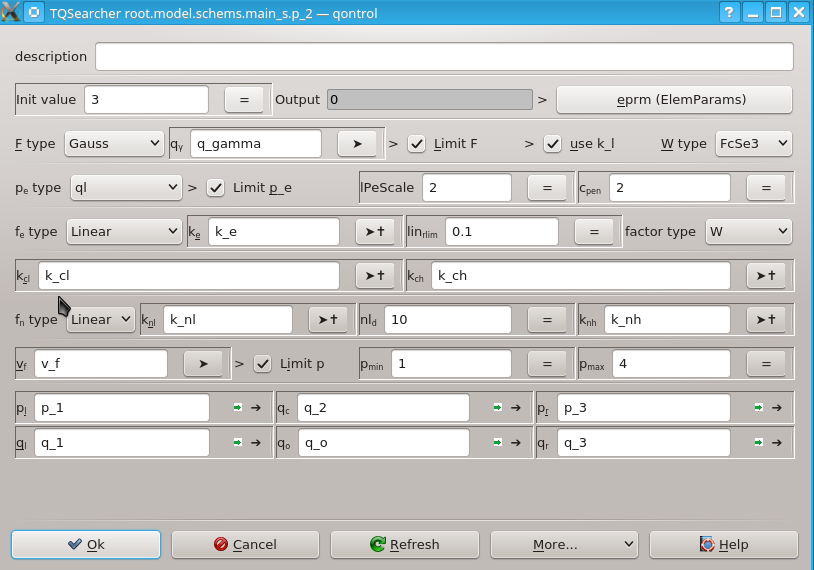
\includegraphics[width=0.7\textwidth]{p/qontrol_tqsearch.png}
  \end{center}
\caption{Діалогове вікно з елементами інтерфейсу, автоматично створеними для об'єкта ``TQSearcher''}
  \label{atu:f:qontrol_qsearch}
\end{figure}

Для забезпечення сигнального і параметричного зв'язку
між елементами системи, що моделюється, створено класи
LinkedObj, InputAbstract, InputSimple, InputLogic, ParamDouble. Клас LinkedObj дозволяє
реалізовувати зв'язок між елементами в момент виконання,
причому з мінімальними накладними витратами, на рівні
доступу за покажчиком. Будь-який клас, що може бути джерелом
даних, повинен бути його відкритим спадкоємцем. При цьому
автоматично враховується ієрархічна структура і доступ
до вкладених елементів.

У якості структурного елементу, який є
приймачем даних, може виступати спадкоємець InputAbstract. Об'єкти
типу InputSimple реалізують простий сигнальний зв'язок. Джерелом
може бути будь-який елемент схеми, параметр моделі в цілому,
поточної задачі моделювання, просто константа. При цьому кожен
такий вхід має незалежний множник і зміщення, а також параметри
відображення на схемі моделі~(рис.~\ref{atu:f:qontrol_link}).


\begin{figure}[htb!]
  \begin{center}
    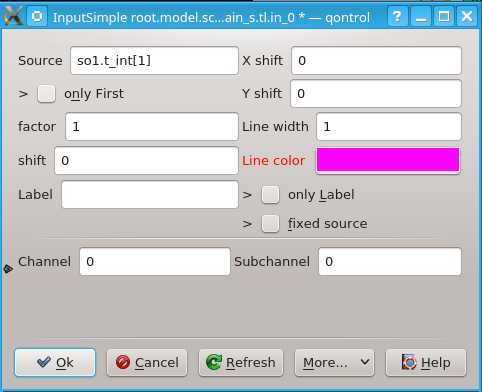
\includegraphics[width=0.5\textwidth]{p/qontrol_link.png}
  \end{center}
\caption{Діалогове вікно для редагування елемента типу InputSimple, для визначення параметрів сигнального зв'язку між об'єктами}
  \label{atu:f:qontrol_link}
\end{figure}

Для тих елементів, які потребують наявності змінної
кількості входів, наприклад, координатора пошуку, важливими
параметрами входів є ``channel'' і ``subchannel'', що задають відповідно
номер вхідного каналу і субканалу. Для координатора пошуку
номер каналу задає номер відповідного агента, а номер субканалу
--- величини $ p_e $ і $ F $ відповідно.

Деякі зв'язки являють собою логічні величини, наприклад, сигнали
дозволу роботи елемента, вхідні сигнали для лічильників,
тригерів і подібних. Для їх обробки створено окремий клас ---
InputLogic. Примірники цього класу виконують ті ж дії, що і InputSimple,
при цьому сигнал приводиться до логічного виду за заданими
правилами. Крім простого поділу по порогу, реалізовані
можливості використання тригера Шмідта і детектора фронтів.

Для реалізації параметричних входів використовуються
екземпляри класу ParamDouble. Відмінність їх поведінки від
поведінки сигнальних входів полягає в тому, що при зміні
значення параметра, відповідним елементом можуть бути
зроблені певні дії. Якщо ж значенням параметра є константа,
або ж значення параметра зафіксовано при початку процесу
моделювання, то отримання даних відбувається тільки в момент
початку моделювання, що істотно зменшує обчислювальні витрати
на чисельне моделювання.

Базовим класом для всіх елементів, які можуть бути присутніми
в схемі моделі, є TMiso. Він доповнює можливості, що надаються
своїм базовим класом, LinkedObj, діями, які виконуються безпосередньо
в процесі моделювання, перед одним запуском моделювання, перед
групою запусків моделювання, а також після завершення цих
процесів. Всього у класу TMiso близько 50 спадкоємців, починаючи від
простих суматорів, логічних елементів, і закінчуючи складними
елементами для реалізації алгоритмів пошукових агентів.

З усіх спадкоємців TMiso слід зазначити елемент TSubScheme. Від
дозволяє в якості елемента поточної схеми використовувати
іншу схему. Інша схема може бути як частиною моделі, що
зараз використовується, так і завантажуватися з бібліотек
схем. Бібліотеки схем --- це звичайні файли моделей, які містять
іменовані схеми.

Для отримання даних із зовнішніх джерел призначено два
класи: TFileSource і TFileSimple. Обидва дозволяють отримувати дані як
з файлу, в тому числі спеціального, що відображає операції
введення - виведення на зовнішній пристрій або ж інший
процес операційної системи. Перший з них, ціною додаткових
обчислювальних витрат дозволяє проводити передискретизацію
сигналу у часовій області. Другий, за рахунок менших накладних
витрат, є більш підходящим при моделюванні в реальному масштабі
часу.

Об'єкти типу ``Scheme'' призначені для об'єднання елементів моделі,
при цьому вони самі об'єднані у контейнер схем ``schems'' типу ``ContScheme''.
Гарантується наявність як мінімум однієї схеми, у якій
зарезервоване ім'я ``main\_s''. Ця схема є основною при моделюванні,
інші призначені для створення вкладених схем за допомогою
об'єктів типу ``TSubScheme''.

Для збору і обробки даних при моделюванні призначені об'єкти
типу ``TOutArr'', розташовані в контейнері ``outs'' типу ``ContOut''. Кожен з
них може збирати дані з будь-якого елементу моделі, включаючи
параметри моделі, задач моделювання або ж інших таких
же об'єктів. При цьому можна задати шпарування та час отримання
даних, метод отримання та інші параметри. Також об'єкти цього
типу можуть використовуватися як сховища даних для різних
алгоритмів, наприклад статистичного, регресійного або Фур'є
аналізу. Базові статистичні операції, такі як обчислення
діапазону, середнього, дисперсії відбуваються автоматично. Дані
можуть бути експортовані, але основне призначення --- служити
основою для побудови графіків.

Для побудови графіків використовуються об'єкти типу TGraph,
розташовані в контейнері ``plots'' типу ``ContOut''. У кожному з них
міститься об'єкт типу ``SchemeData'', що містить загальну інформацію
про графік, таку як розмір, колірна палітра, правила і обмеження
при побудові осей координат, легенди та інше. Дані, за якими
будуються графіки, визначаються елементами типу ``GraphElem''. Кожен
з них задає джерело даних, а також визначає, як ці дані будуть
використовуватися: як дані для осей координат, двовимірних
або тривимірних графіків різних типів, задають колір або
прозорість. Одночасно можуть бути створені декілька графіків
різних типів, але з осями координат, що збігаються. Відображенням
графіків можна управляти як за допомогою інтерфейсу
користувача, так і за допомогою скриптів.

Крім графіків, на зображенні можуть бути розташовані мітки
(PlotLabel) і найпростіші графічні примітиви (PlotFlippery), причому
координати і тих і інших можуть задаватися на підставі будь-яких
числових параметрів моделі. Текст міток також може визначатися
даними моделі, при цьому є можливість задавати формат даних, що
виводяться. Для виведення спеціальних математичних символів,
букв грецького алфавіту використовується підмножина
математичних команд \LaTeX-а. Крім відображення на графіках,
мітки можуть використовуватися як частина шаблону імені файлу
при експорті зображення, а також зберігатися в якості
метаінформації файлу.

Для відображення графіків використовується Mathgl ---
кроссплатформенная бібліотека для підготовки високоякісних
наукових ілюстрацій. Крім відображення графіків,
відповідні вікна надають набір простих інструментів для
аналізу~\cite{atu_jacs2015}~(рис.~\ref{atu:f:qontrol_3d}).


\begin{figure}[htb!]
  \begin{center}
    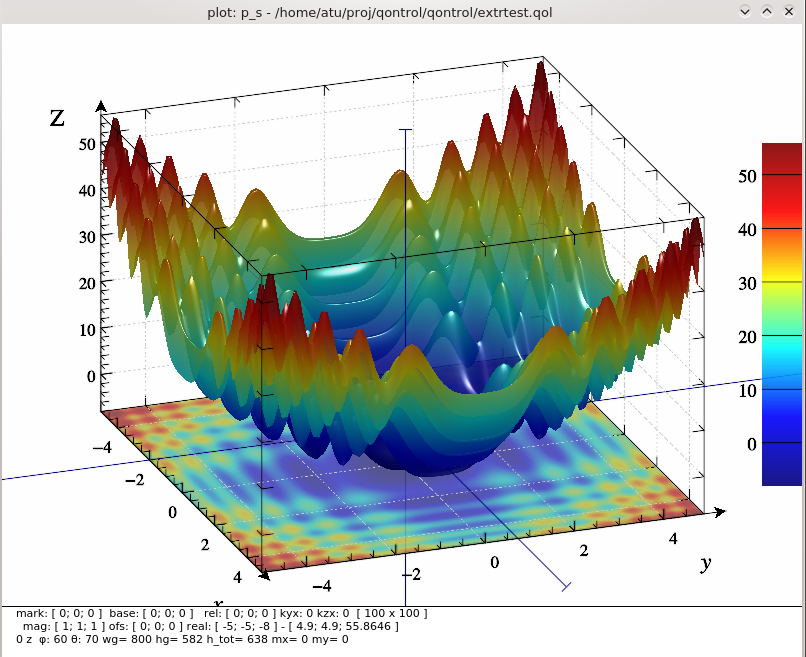
\includegraphics[width=0.7\textwidth]{p/qontrol_3d_a.png}
  \end{center}
\caption{Вікно, призначене для відображення графіків у програмі ``qontrol''}
  \label{atu:f:qontrol_3d}
\end{figure}

Параметри моделювання (симуляції) задаються об'єктами
типу ``Simulation'', розташованими в контейнері ``sims'' типу ``ContSimul''.
Завжди існує об'єкт з ім'ям ``sim0'', що визначає симуляцію за
замовчуванням. Параметри цих об'єктів задають тип моделювання
(просте моделювання, одне і двох параметрична ітерація), повний
час і крок моделювання, імена функцій скриптів, що викликаються на
різних стадіях, а також довільний набір параметрів, типи, імена
і значення яких задає користувач~(рис.~\ref{atu:f:qontrol_simul}). Модель
може містити довільну кількість стимуляцій, але одночасно
виконуватися може тільки одна.

\begin{figure}[htb!]
  \begin{center}
    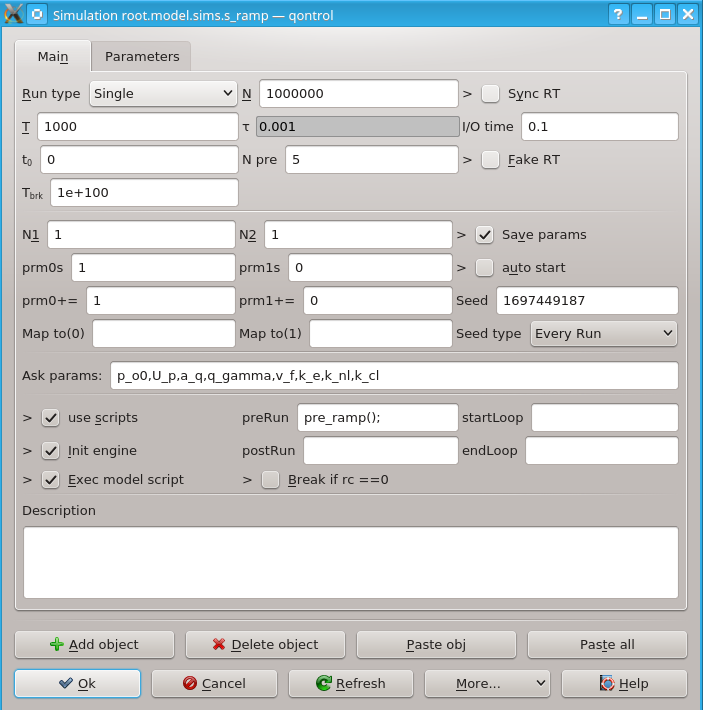
\includegraphics[width=0.7\textwidth]{p/qontrol_task.png}
  \end{center}
\caption{Діалогове вікно, призначене для завдання параметрів моделювання (Simulation)}
  \label{atu:f:qontrol_simul}
\end{figure}


Центральний об'єкт, який об'єднує всю ієрархію моделі,
називається ``model'' і має тип ``TModel''. Крім уже згаданих контейнерів
``schems'', ``outs'', ``sims'', ``schems'', цей об'єкт містить свій довільний
набір параметрів. При моделюванні, параметри симуляції
мають пріоритет над параметрами моделі, що дозволяє гнучко
управляти наборами параметрів при проведенні обчислювальних
експериментів.

Об'єкт ``model'' також містить елемент ``script'', який може містити
використовувані в процесі моделювання скрипти в вигляді функцій
на мові JavaScript. При моделюванні всі об'єкти, які беруть участь в
процесі, імпортуються в поточну область видимості під своїми
іменами~(рис. \ref{atu:f:qontrol_js}).


\begin{figure}[htb!]
  \begin{center}
    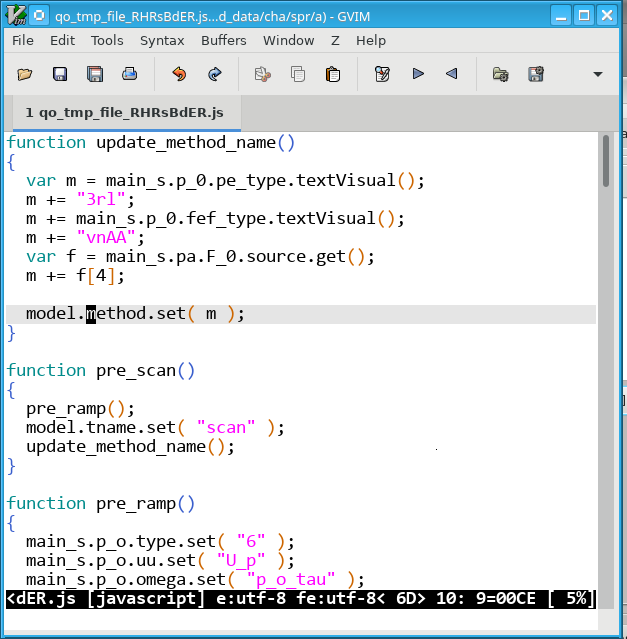
\includegraphics[width=0.6\textwidth]{p/qontrol_js.png}
  \end{center}
\caption{Приклад скриптів програми ``qontrol''}
  \label{atu:f:qontrol_js}
\end{figure}



% }}}2




% }}}1

\section{Інтерфейс користувача програмного комплексу} % {{{1 ------------------------------------- ---

Інтерфейс програми ``qontrol'' був створений за допомогою засобів,
що надаються бібліотекою Qt. Використовується класичний
MDI інтерфейс, тобто для кожної моделі створюється окреме
вікно, яке відображає структуру моделі, і дозволяє її
змінювати~(рис.~\ref{atu:f:qontrol_all}). Крім основного вікна, для кожної
моделі може бути відкрити довільне число вікон відображення
графіків і редагування субсхем.


\begin{figure}[htb!]
  \begin{center}
    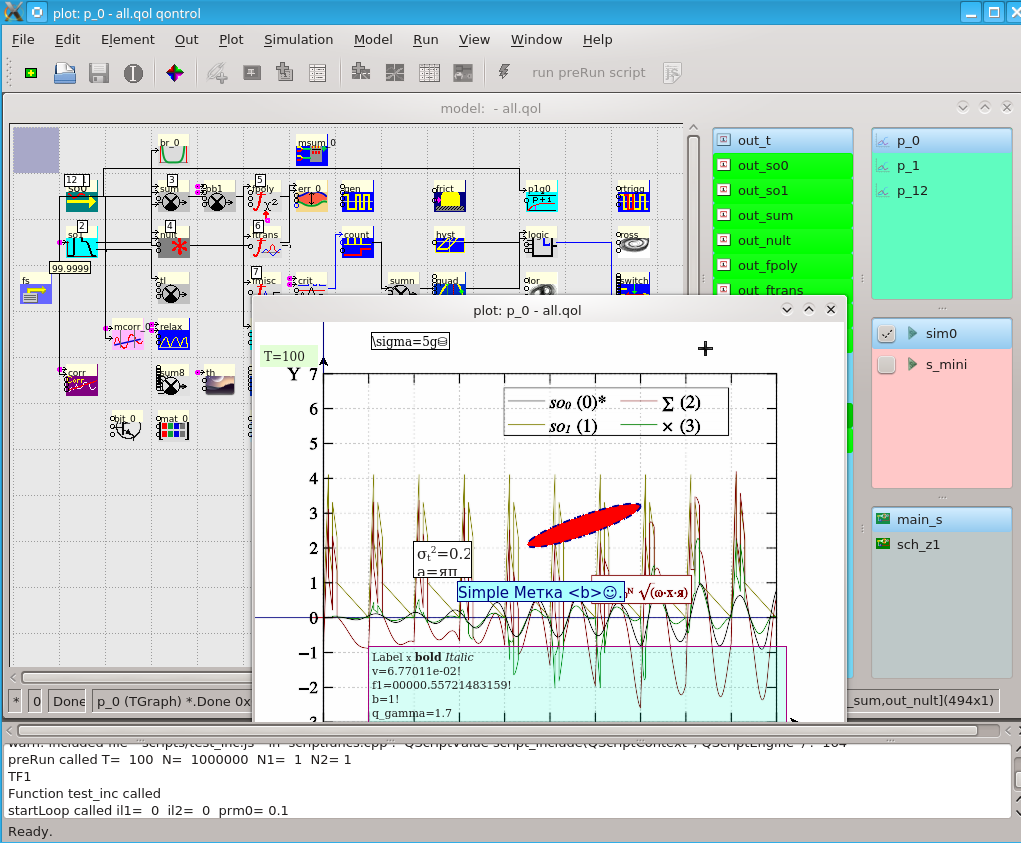
\includegraphics[width=0.96\textwidth]{p/qontrol_all.png}
  \end{center}
\caption{Загальний вигляд інтерфейсу користувача програми ``qontrol''}
  \label{atu:f:qontrol_all}
\end{figure}

Центральну частину вікна займає редактор основної схеми
моделі. Після моделювання там також можуть бути відображені
довільні дані, пов'язані з елементами моделі.

У правій частині вікна розташовані списки об'єктів збору даних,
графіків, параметрів моделювання і схем. Нижню частину вікна
займає область виведення, в яку надходять повідомлення про
помилки, зауваження, а також стандартний потік виводу скриптів.


Файли моделей зберігаються в XML форматі з суфіксом ``.qol'', що дає
можливість їх редагувати за межами програми як за допомогою
звичайних текстових редакторів, так і з використанням
спеціальних засобів для обробки структурованих XML документів.


Програма може бути запущена і без графічного інтерфейсу. При
цьому обов'язкова вказівка в командному рядку імені
моделі. Додатково вказується ім'я симуляції, задаються параметри
моделювання, і, при необхідності, вказівки про те, куди і як
зберігати отримані дані і створені графіки.

% }}}1


\section{Висновки по розділу \thechapter} % {{{1 ----------------------------------- ----------

Створено програмне середовище ``qontrol'', що призначено для
моделювання нелінійних динамічних систем, має набір якостей,
які суттєво спрощують процес моделювання, створення нових
систем ідентифікації та управління. До характеристик програми
слід віднести:

\begin{itemize}

  \item
    Універсальність, що дозволяє створювати моделі складних
    динамічних систем, з можливістю комбінування і угруповання
    елементів системи.

  \item
    Розвинені засоби обробки і представлення даних.

  \item
    Зручний інтерфейс користувача.

  \item
    Висока швидкість моделювання.

  \item
    Можливість запускати програму в командному режимі, без
    графічного інтерфейсу для проведення моделювання в пакетному
    режимі.

  \item
    Автоматична побудова інтерфейсу користувача на основі даних,
    що подаються елементом.

  \item
    Можливість реалізації складних задач моделювання, які не
    вписуються в набір базових дій, за рахунок застосування
    вбудованої мови програмування, заснованої на JavaScript, з
    можливістю доступу до функцій програмного середовища.

  \item
    Широкі можливості по відображенню інформації в графічному
    вигляді.

  \item
    Можливість взаємодії з іншими програмними і
    апаратно-програмними комплексами.


  \item
    Відкритий вихідний код, що дає можливість як застосовувати
    елементи створеної програми в своїх розробках, так і доповнювати
    програму своїми елементами.


  \item
    Open-source ліцензія і вільне поширення, що дозволяє без істотних
    витрат використовувати програмне середовище при проведенні
    досліджень і в навчальному процесі.

\end{itemize}

Список використаних джерел у даному розділі наведено у повному
списку використаних джерел під номерами
\cite{atu_asau26},
\cite{atu_asau26},
\cite{atu_jacs2015}

% }}}1


% vim: fdm=marker ft=tex
